\documentclass[12pt]{article}

\usepackage{blindtext} % Package to generate dummy text throughout this template 

\usepackage[utf8]{inputenc}
\usepackage{amsmath, amssymb}
%\usepackage{times} % Use the Times font
%\usepackage[T1]{fontenc}
\linespread{1.25}
\usepackage[margin = 1in]{geometry}
\usepackage{microtype} % Slightly tweak font spacing for aesthetics
\usepackage[english]{babel} % Language hyphenation and typographical rules
\usepackage{tikz}
\usepackage{hyperref}
\usepackage{url}

\tikzset{mynode/.style={font=\footnotesize,inner sep=0pt,text=black}
}
\setlength{\parindent}{2em}
%\setlength{\parskip}{1.5em}

\newcommand{\vect}[1]{\mathbf{#1}}
\newcommand{\matr}[1]{\mathbf{#1}}
\newcommand{\mean}[1]{\overline{#1}}

    \pgfdeclarelayer{x2}
\pgfdeclarelayer{x3}
\pgfdeclarelayer{x4}
\pgfsetlayers{x4, x3, x2, main}  % set the order of the layers (main is the standard layer)

\begin{document}
    \tableofcontents
    \section{Introduction} \label{introduction}
    Optimizing predictive models datasets obtained from citizen science projects can be computationally expensive due to limited parallelism offered by Central Processing Units (CPUs). Since these crowd-sourced datasets grow with time as the researchers warrant more information, running models can prove increasingly difficult even on the fastest CPUs available in the market. However, Graphical Processing Units (GPUs), which offer multiple cores to parallelize computation, can outperform CPUs in computing such predictive models given the operations are arithmetically simple (though large in number) and boolean logic-free to the maximum extent.\\
    
    One such predictive model is Avicaching \cite{Xue2016Avi1} in the eBird platform [cite], which aims to ``maximize the utility and accessibility of the vast numbers of bird observations made each year by recreational and professional bird watchers'' [cite website]. Since the eBird dataset is heterogeneous geographically, Avicaching tries to homogenize future observations by providing observer-citizens incentives to visit under-sampled locations \cite{Xue2016Avi1}. Therefore, the Avicaching game can be modeled as two separate problems - identifying parameters of citizens' behavior on a specific set of rewards (incentives), and pooling rewards from a budget to locations such that the citizens' predicted behavior is homogeneous \cite{Xue2016Avi2}.
    
    \subsection{Identification Problem} \label{iden_problem}
    This subroutine will learn parameters of the change in citizens' behavior due to rewards. Specifically, given datasets $\vect{y_t}$ and $\vect{x_t}$ of citizens' visit densities with and without the rewards $\vect(r_t)$, we want to find weights $\matr{w}$ that caused the change from $\vect{x_t}$ to $\vect{y_t}$, factoring in possible influence due to environmental factors $\matr{f}$. Therefore, the model is:
    \begin{equation}
    \begin{aligned}
    & \underset{\matr{w}}{\text{minimize}}
    & & Z_I(\matr{w}) = \sum_{t} (u_t(\vect{y_t} - P(\matr{f}, \vect{r_t}; \matr{w})\vect{x_t}))^{2}
    \end{aligned}
    \end{equation}
    where $u_t$ is the total number of submissions at time $t$ for a given citizen and elements $p_{u, v}$ of $P$ are given as:
    \begin{equation} \label{puv_equation}
    p_{u, v} = \frac{\exp{(\matr{w} \cdot [\vect{f_{u, v}}, r_{u}])}}{\sum_{u'} \exp{(\matr{w} \cdot [\vect{f_{u', v}}, r_{u'}])}}
    \end{equation}
    
    \subsection{Pricing Problem} \label{pricing_problem}
    The Pricing subroutine will attempt to allocate rewards to all locations such that the predicted behavior is least heterogeneous, given the learned parameters from Section \ref{iden_problem}. This optimization problem can be written as:
    \begin{equation}
    \begin{aligned}
    & \underset{\vect{r}}{\text{minimize}}
    & & Z_P(\vect{r}) = \frac{1}{n}\lVert \vect{y} - \mean{\vect{y}} \rVert\\
    & \text{subject to}
    & & \vect{y} = P(\matr{f}, \vect{r}; \matr{w}) \, \vect{x}\\
    &&& \sum_{i} r_i \leq \mathcal{R}\\
    &&& r_i \geq 0
    \end{aligned}
    \end{equation}
    where $\mathcal{R}$ is total reward budget and $P$ is defined as in Equation \ref{puv_equation}.
    
    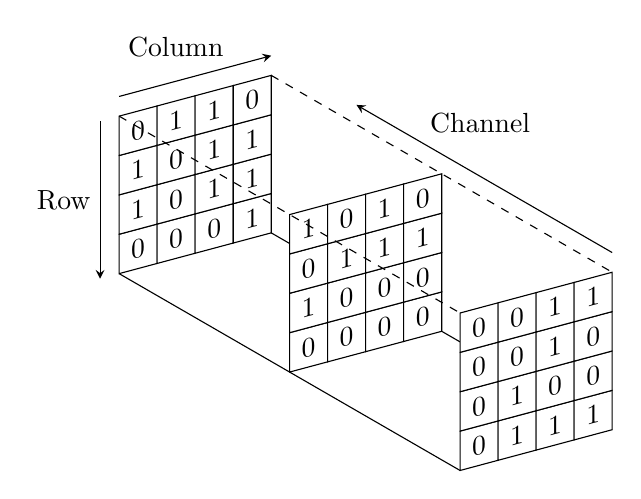
\begin{tikzpicture}[x=(15:.5cm), y=(90:.5cm), z=(330:.5cm), >=stealth]
    \draw (0, 0, 0) -- (0, 0, 10) (4, 0, 0) -- (4, 0, 10);
    \foreach \z in {0, 5, 10} \foreach \x in {0,...,3}
    \foreach \y [evaluate={\b=random(0, 1);}] in {0,...,3}
    \filldraw [fill=white] (\x, \y, \z) -- (\x+1, \y, \z) -- (\x+1, \y+1, \z) --
    (\x, \y+1, \z) -- cycle (\x+.5, \y+.5, \z) node [yslant=tan(15)] {\b};
    \draw [dashed] (0, 4, 0) -- (0, 4, 10) (4, 4, 0) -- (4, 4, 10);
    \draw [->] (0, 4.5, 0)  -- (4, 4.5, 0)   node [near end, above left] {Column};
    \draw [->] (-.5, 4, 0)  -- (-.5, 0, 0)   node [midway, left] {Row};
    \draw [->] (4, 4.5, 10) -- (4, 4.5, 2.5) node [near end, above right] {Channel};
    \end{tikzpicture}
    
    \subsection{Computation Using GPUs} \label{comp_using_GPUs}
    
    \section{Problem Formulation}
    Since NVIDIA General Purpose GPUs enable faster computation on matrices, accelerated through CUDA and cuDNN, both the Identification Problem (Section \ref{iden_problem}) and Pricing Problem (Section \ref{pricing_problem}) were formulated as 2-layer Neural Networks using the PyTorch platform.
    
    \subsection{Design for Identification Problem}
    
    \tikzset{
        every neuron/.style={
            circle,
            shading=ball,
            ball color=gray!40,
            %opacity=0.4,
            draw,
            minimum size=1cm
        },
        neuron missing/.style={
            draw=none,
            shading=none, 
            scale=4,
            text height=0.333cm,
            execute at begin node=\color{black}$\vdots$
        },
    }
    
    \begin{tikzpicture}[x=(15:1.5cm), y=(90:1.5cm), z=(350:1.5cm), >=stealth]
    
    \foreach \m [count=\y] in {1, 2, 3, missing, 4} {
        \node [every neuron/.try, neuron \m/.try] (input-1\m) at (0, 2.5-\y, 0) {};
    }

    \begin{pgfonlayer}{x2}
    \foreach \m [count=\y] in {1, 2, 3, missing, 4} {
        \node [every neuron/.try, neuron \m/.try] (input-2\m) at (1, 2.5-\y, 0) {};
    }
    \end{pgfonlayer}
    \foreach \i [count=\x] in {1, 2, 3, 4} {
        %\shade[ball color=gray!40, opacity=0.4] (\x-2.5, 0, 5) circle (0.5cm);
        %\draw (\x-2.5, 0, 5) circle (0.5cm) {input-\x\y};
        \node [every neuron] (output-\x) at (\x-2.5, 0, 5) {};
    }
    %\foreach \m [count=\y] in {1,2,3,missing,4}
    %\node [every neuron/.try, neuron \m/.try] (input-\m) at (0,-\y, 0) {};
    
    %\foreach \m [count=\y] in {1,missing,2}
    %\node [every neuron/.try, neuron \m/.try ] (hidden-\m) at (2,2-\y*1.25) {};
    
    %\foreach \m [count=\y] in {1,missing,2}
    %\node [every neuron/.try, neuron \m/.try ] (output-\m) at (4,1.5-\y) {};
    
    %\foreach \l [count=\i] in {1,2,3,n}
    %\draw [<-] (input-\i) -- ++(-1,0)
    %node [above, midway] {$I_\l$};
    
    %\foreach \l [count=\i] in {1,n}
    %\node [above] at (hidden-\i.north) {$H_\l$};
    
    %\foreach \l [count=\i] in {1,n}
    %\draw [->] (output-\i) -- ++(1,0)
    %node [above, midway] {$O_\l$};
    
    \foreach \x in {1, ..., 4}
        \foreach \y in {1,...,4}
            \draw [->] (input-\x\y) -- (output-\x);
    
    %\foreach \i in {1,...,2}
    %\foreach \j in {1,...,2}
    %\draw [->] (hidden-\i) -- (output-\j);
    
    %\foreach \l [count=\x from 0] in {Input, Hidden, Ouput}
    %\node [align=center, above] at (\x*2,2) {\l \\ layer};
    
    \end{tikzpicture}
    
    \section{Experiments}
    \section{Results}
    \section{Conclusion}
    \blindtext
    \bibliographystyle{ieeetr}
    \bibliography{avicaching}
\end{document}